% Standalone source of the figure fig:poisson of the continuum-limit paper.
% Build: pdflatex fig_poisson.tex (or lualatex); the paper includes the PDF.
\documentclass[border=2pt]{standalone}
% Shared preamble of the continuum-limit paper's standalone figures.
\usepackage{amsmath,amssymb,bm}
\usepackage{tikz}
\usetikzlibrary{calc}
\newcommand{\bS}{\mathbf{S}}
\newcommand{\bG}{\mathbf{G}}
\newcommand{\bK}{\mathbf{K}}
\newcommand{\bP}{\mathbf{P}}
\newcommand{\sinc}{\operatorname{sinc}}

\begin{document}
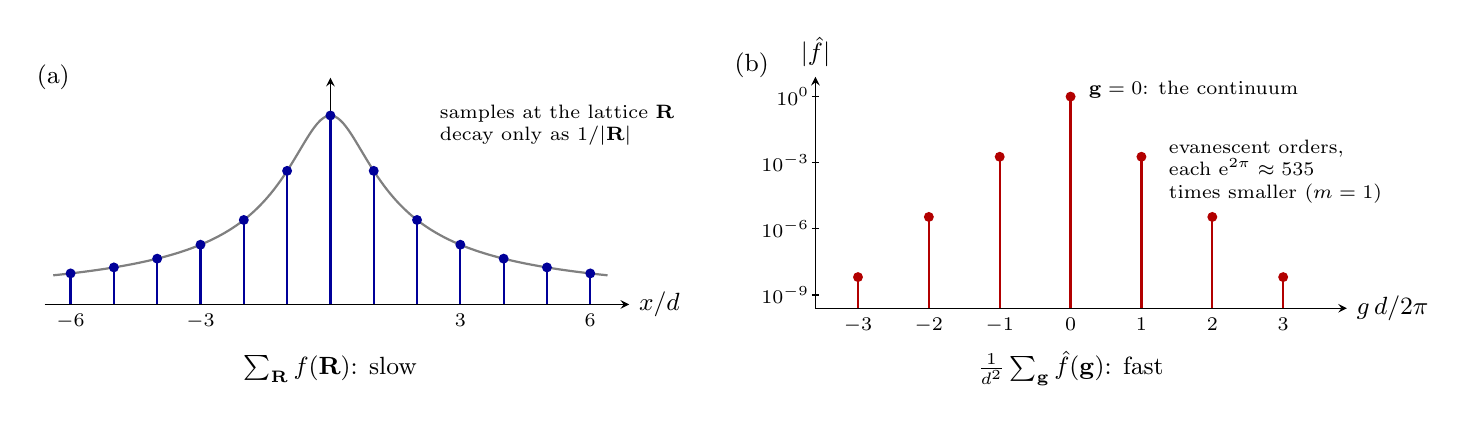
\begin{tikzpicture}[>=stealth, font=\small]
  % (a) real space: samples of the field of a plane of voxels at the lattice points, decaying slowly
  \begin{scope}[x=0.55cm, y=2.4cm]
    \draw[->] (-6.6,0) -- (6.9,0) node[right] {$x/d$};
    \draw[->] (0,0) -- (0,1.2);
    \draw[thick, gray, domain=-6.4:6.4, samples=200, smooth] plot (\x, {1/sqrt(\x*\x+1)});
    \foreach \r in {-6,...,6} {
      \draw[blue!60!black, thick] (\r,0) -- (\r,{1/sqrt(\r*\r+1)});
      \fill[blue!60!black] (\r,{1/sqrt(\r*\r+1)}) circle (1.8pt);
    }
    \foreach \r in {-6,-3,3,6} \node[below, font=\scriptsize] at (\r,0) {$\r$};
    \node[align=left, font=\scriptsize, right] at (2.3,0.95) {samples at the lattice $\mathbf R$\\decay only as $1/|\mathbf R|$};
    \node at (-6.4,1.2) {(a)};
    \node[below] at (0,-0.22) {$\sum_{\mathbf R}f(\mathbf R)$: slow};
  \end{scope}
  % (b) reciprocal space, log scale: the continuum order and the evanescent orders, each e^{2 pi} smaller
  \begin{scope}[shift={(9.4,2.64)}, x=0.9cm, y=0.28cm]
    \draw[->] (-3.6,-9.6) -- (3.9,-9.6) node[right] {$g\,d/2\pi$};
    \draw[->] (-3.6,-9.6) -- (-3.6,0.9) node[above] {$|\hat f|$};
    \foreach \e in {0,-3,-6,-9} \draw (-3.65,\e) -- (-3.55,\e) node[left, font=\scriptsize] {$10^{\e}$};
    \foreach \p in {-3,...,3} {
      \pgfmathsetmacro{\h}{-2*pi*abs(\p)/ln(10)}
      \draw[thick, red!70!black] (\p,-9.6) -- (\p,\h);
      \fill[red!70!black] (\p,\h) circle (1.8pt);
      \node[below, font=\scriptsize] at (\p,-9.6) {$\p$};
    }
    \node[right, font=\scriptsize] at (0.12,0.3) {$\mathbf g=0$: the continuum};
    \node[right, align=left, font=\scriptsize] at (1.25,-3.4) {evanescent orders,\\each $\mathrm{e}^{2\pi}\approx535$\\times smaller ($m=1$)};
    \node at (-4.5,1.4) {(b)};
    \node[below] at (0,-11.1) {$\frac1{d^2}\sum_{\mathbf g}\hat f(\mathbf g)$: fast};
  \end{scope}
\end{tikzpicture}
\end{document}
